% Options for packages loaded elsewhere
\PassOptionsToPackage{unicode}{hyperref}
\PassOptionsToPackage{hyphens}{url}
\PassOptionsToPackage{dvipsnames,svgnames,x11names}{xcolor}
%
\documentclass[
  letterpaper,
  DIV=11,
  numbers=noendperiod]{scrartcl}

\usepackage{amsmath,amssymb}
\usepackage{iftex}
\ifPDFTeX
  \usepackage[T1]{fontenc}
  \usepackage[utf8]{inputenc}
  \usepackage{textcomp} % provide euro and other symbols
\else % if luatex or xetex
  \usepackage{unicode-math}
  \defaultfontfeatures{Scale=MatchLowercase}
  \defaultfontfeatures[\rmfamily]{Ligatures=TeX,Scale=1}
\fi
\usepackage{lmodern}
\ifPDFTeX\else  
    % xetex/luatex font selection
\fi
% Use upquote if available, for straight quotes in verbatim environments
\IfFileExists{upquote.sty}{\usepackage{upquote}}{}
\IfFileExists{microtype.sty}{% use microtype if available
  \usepackage[]{microtype}
  \UseMicrotypeSet[protrusion]{basicmath} % disable protrusion for tt fonts
}{}
\makeatletter
\@ifundefined{KOMAClassName}{% if non-KOMA class
  \IfFileExists{parskip.sty}{%
    \usepackage{parskip}
  }{% else
    \setlength{\parindent}{0pt}
    \setlength{\parskip}{6pt plus 2pt minus 1pt}}
}{% if KOMA class
  \KOMAoptions{parskip=half}}
\makeatother
\usepackage{xcolor}
\setlength{\emergencystretch}{3em} % prevent overfull lines
\setcounter{secnumdepth}{5}
% Make \paragraph and \subparagraph free-standing
\ifx\paragraph\undefined\else
  \let\oldparagraph\paragraph
  \renewcommand{\paragraph}[1]{\oldparagraph{#1}\mbox{}}
\fi
\ifx\subparagraph\undefined\else
  \let\oldsubparagraph\subparagraph
  \renewcommand{\subparagraph}[1]{\oldsubparagraph{#1}\mbox{}}
\fi


\providecommand{\tightlist}{%
  \setlength{\itemsep}{0pt}\setlength{\parskip}{0pt}}\usepackage{longtable,booktabs,array}
\usepackage{calc} % for calculating minipage widths
% Correct order of tables after \paragraph or \subparagraph
\usepackage{etoolbox}
\makeatletter
\patchcmd\longtable{\par}{\if@noskipsec\mbox{}\fi\par}{}{}
\makeatother
% Allow footnotes in longtable head/foot
\IfFileExists{footnotehyper.sty}{\usepackage{footnotehyper}}{\usepackage{footnote}}
\makesavenoteenv{longtable}
\usepackage{graphicx}
\makeatletter
\def\maxwidth{\ifdim\Gin@nat@width>\linewidth\linewidth\else\Gin@nat@width\fi}
\def\maxheight{\ifdim\Gin@nat@height>\textheight\textheight\else\Gin@nat@height\fi}
\makeatother
% Scale images if necessary, so that they will not overflow the page
% margins by default, and it is still possible to overwrite the defaults
% using explicit options in \includegraphics[width, height, ...]{}
\setkeys{Gin}{width=\maxwidth,height=\maxheight,keepaspectratio}
% Set default figure placement to htbp
\makeatletter
\def\fps@figure{htbp}
\makeatother

\KOMAoption{captions}{tableheading}
\makeatletter
\@ifpackageloaded{caption}{}{\usepackage{caption}}
\AtBeginDocument{%
\ifdefined\contentsname
  \renewcommand*\contentsname{Table of contents}
\else
  \newcommand\contentsname{Table of contents}
\fi
\ifdefined\listfigurename
  \renewcommand*\listfigurename{List of Figures}
\else
  \newcommand\listfigurename{List of Figures}
\fi
\ifdefined\listtablename
  \renewcommand*\listtablename{List of Tables}
\else
  \newcommand\listtablename{List of Tables}
\fi
\ifdefined\figurename
  \renewcommand*\figurename{Figure}
\else
  \newcommand\figurename{Figure}
\fi
\ifdefined\tablename
  \renewcommand*\tablename{Table}
\else
  \newcommand\tablename{Table}
\fi
}
\@ifpackageloaded{float}{}{\usepackage{float}}
\floatstyle{ruled}
\@ifundefined{c@chapter}{\newfloat{codelisting}{h}{lop}}{\newfloat{codelisting}{h}{lop}[chapter]}
\floatname{codelisting}{Listing}
\newcommand*\listoflistings{\listof{codelisting}{List of Listings}}
\makeatother
\makeatletter
\makeatother
\makeatletter
\@ifpackageloaded{caption}{}{\usepackage{caption}}
\@ifpackageloaded{subcaption}{}{\usepackage{subcaption}}
\makeatother
\ifLuaTeX
  \usepackage{selnolig}  % disable illegal ligatures
\fi
\usepackage{bookmark}

\IfFileExists{xurl.sty}{\usepackage{xurl}}{} % add URL line breaks if available
\urlstyle{same} % disable monospaced font for URLs
\hypersetup{
  pdftitle={STA302 Project},
  pdfauthor={First author; Another author},
  colorlinks=true,
  linkcolor={blue},
  filecolor={Maroon},
  citecolor={Blue},
  urlcolor={Blue},
  pdfcreator={LaTeX via pandoc}}

\title{STA302 Project\thanks{Code and data are available at:
https://github.com/Yuki010305/Final-Paper.}}
\usepackage{etoolbox}
\makeatletter
\providecommand{\subtitle}[1]{% add subtitle to \maketitle
  \apptocmd{\@title}{\par {\large #1 \par}}{}{}
}
\makeatother
\subtitle{What factors and how influence Ames Iowa Housing Sale Price}
\author{First author \and Another author}
\date{March 31, 2024}

\begin{document}
\maketitle
\begin{abstract}
First sentence. Second sentence. Third sentence. Fourth sentence.
\end{abstract}

\section{Introduction}\label{introduction}

The housing issue is a pillar industry of a country, and the healthy
development of the housing issue affects the country's economic
development level. In order to help the stable development of the
housing transaction market, this project plans to better evaluate the
value of housing transactions for Ames. So, the main purpose of this
project is to explore the factors that influence the sale price of homes
in Ames, Iowa, and how they affect the home sales price. The
characteristics of the homes we selected include central air condition,
car capacity of garage, general shape of property, rate of overall
quality, total above ground living area, number of fireplaces and sale
year. The remainder of this paper is structured as follows.
Section~\ref{sec-data}\ldots.

\section{Data}\label{sec-data}

\begin{verbatim}
  Garage.Cars     Overall.Qual    TotRms.AbvGrd     Gr.Liv.Area  
 Min.   :0.000   Min.   : 1.000   Min.   : 2.000   Min.   : 334  
 1st Qu.:1.000   1st Qu.: 5.000   1st Qu.: 5.000   1st Qu.:1126  
 Median :2.000   Median : 6.000   Median : 6.000   Median :1442  
 Mean   :1.767   Mean   : 6.095   Mean   : 6.443   Mean   :1500  
 3rd Qu.:2.000   3rd Qu.: 7.000   3rd Qu.: 7.000   3rd Qu.:1742  
 Max.   :5.000   Max.   :10.000   Max.   :15.000   Max.   :5642  
  Garage.Area       Fireplaces        Yr.Sold       SalePrice     
 Min.   :   0.0   Min.   :0.0000   Min.   :2006   Min.   : 12789  
 1st Qu.: 320.0   1st Qu.:0.0000   1st Qu.:2007   1st Qu.:129500  
 Median : 480.0   Median :1.0000   Median :2008   Median :160000  
 Mean   : 472.8   Mean   :0.5995   Mean   :2008   Mean   :180806  
 3rd Qu.: 576.0   3rd Qu.:1.0000   3rd Qu.:2009   3rd Qu.:213500  
 Max.   :1488.0   Max.   :4.0000   Max.   :2010   Max.   :755000  
\end{verbatim}

\begin{verbatim}

   N    Y 
 196 2733 
\end{verbatim}

\begin{verbatim}

         N          Y 
0.06691704 0.93308296 
\end{verbatim}

\begin{verbatim}

 IR1  IR2  IR3  Reg 
 979   76   16 1858 
\end{verbatim}

\begin{verbatim}

        IR1         IR2         IR3         Reg 
0.334243769 0.025947422 0.005462615 0.634346193 
\end{verbatim}

\begin{figure}[H]

{\centering 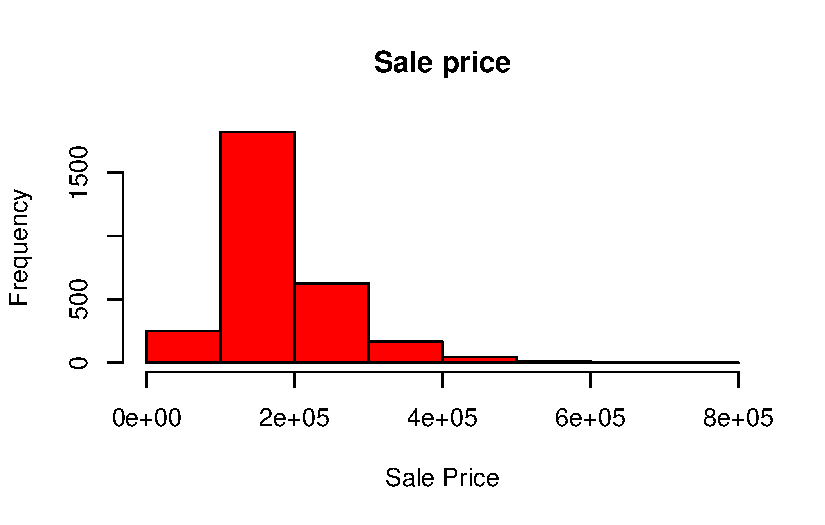
\includegraphics{paper_files/figure-pdf/histprice-1.pdf}

}

\caption{sale price hist}

\end{figure}%

\begin{figure}[H]

{\centering 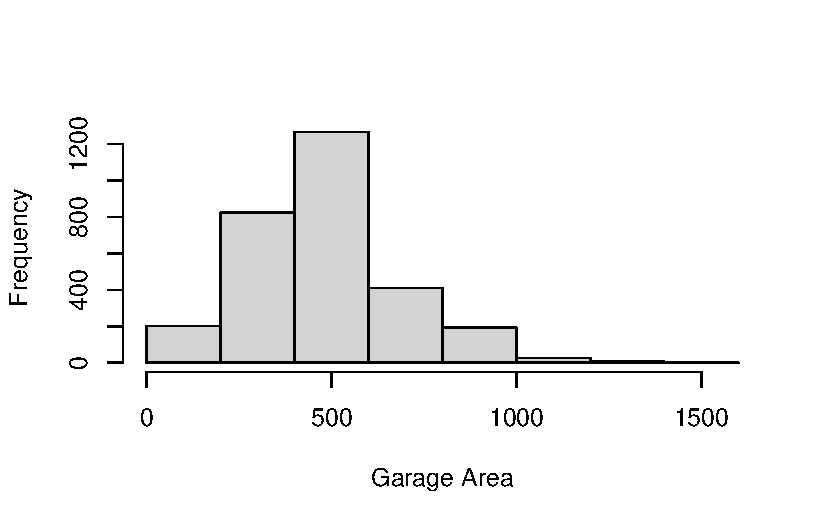
\includegraphics{paper_files/figure-pdf/histbox-1.pdf}

}

\caption{hists}

\end{figure}%

\begin{figure}[H]

{\centering 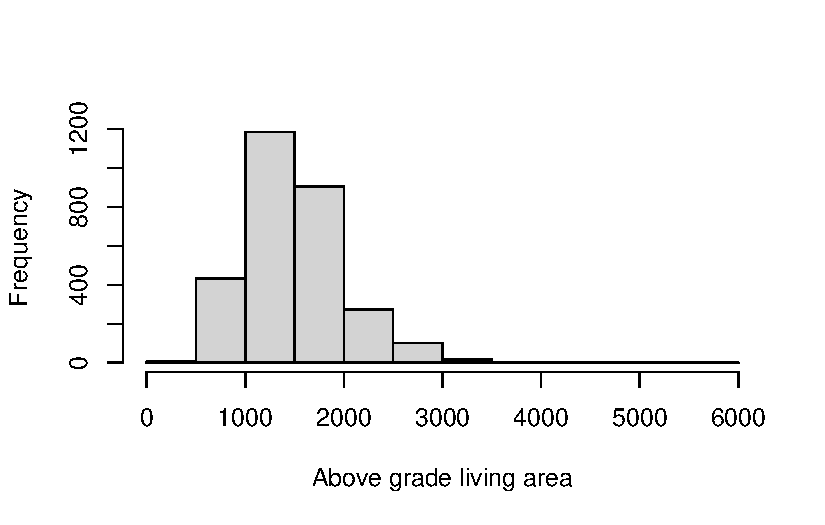
\includegraphics{paper_files/figure-pdf/histbox-2.pdf}

}

\caption{hists}

\end{figure}%

\begin{figure}[H]

{\centering 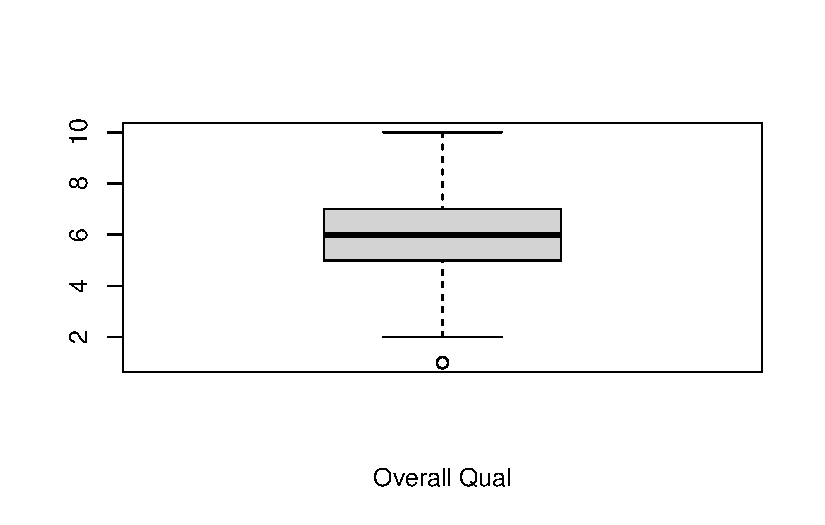
\includegraphics{paper_files/figure-pdf/histbox-3.pdf}

}

\caption{hists}

\end{figure}%

\begin{figure}[H]

{\centering 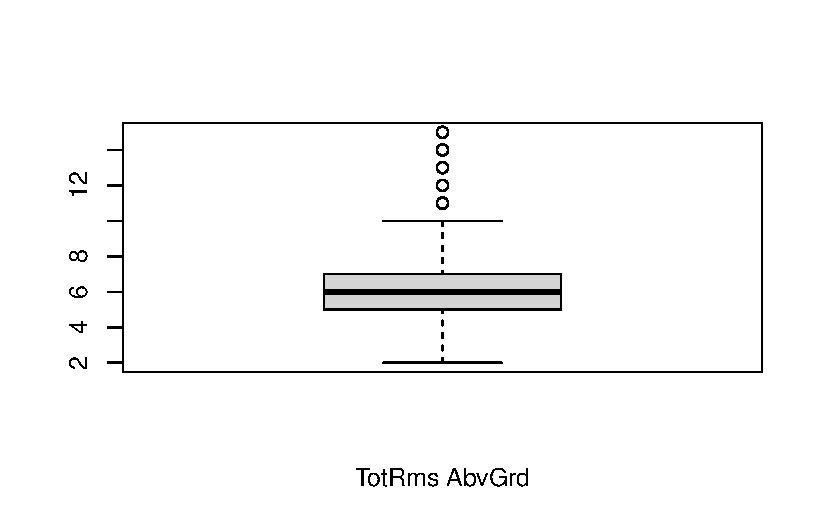
\includegraphics{paper_files/figure-pdf/histbox-4.pdf}

}

\caption{hists}

\end{figure}%

\begin{figure}[H]

{\centering 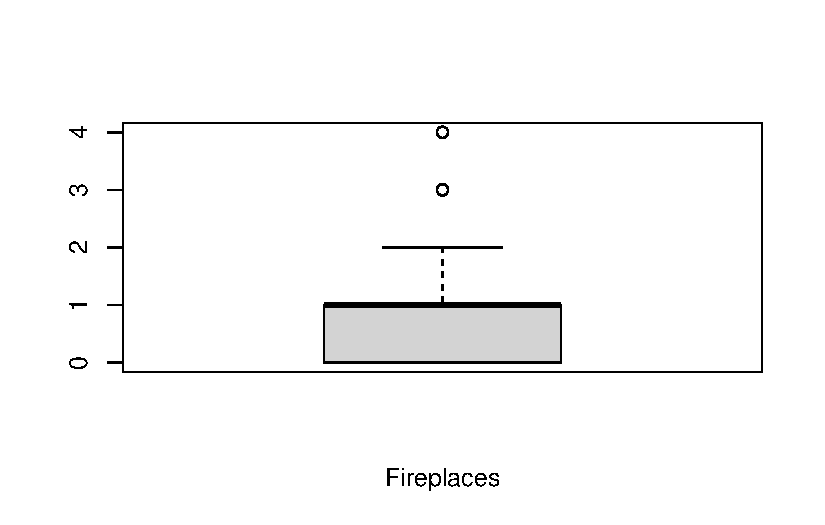
\includegraphics{paper_files/figure-pdf/histbox-5.pdf}

}

\caption{hists}

\end{figure}%

\begin{verbatim}
`geom_smooth()` using formula = 'y ~ x'
`geom_smooth()` using formula = 'y ~ x'
\end{verbatim}

\begin{figure}[H]

{\centering 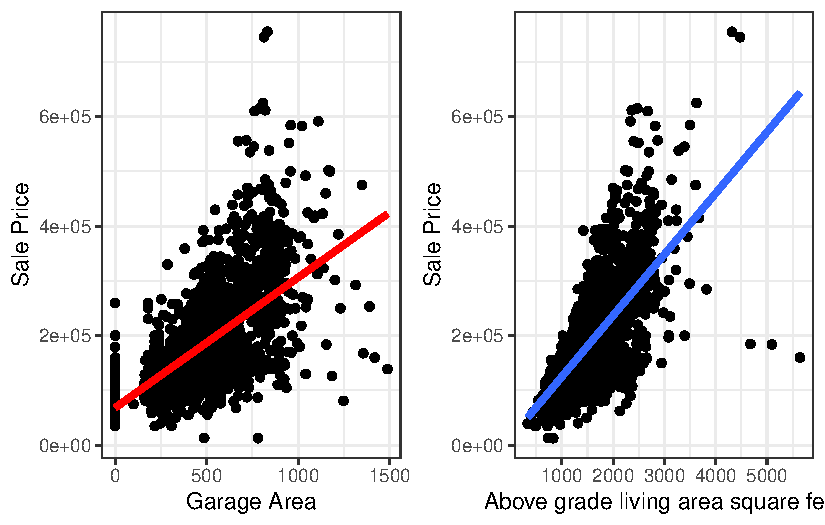
\includegraphics{paper_files/figure-pdf/point-1.pdf}

}

\caption{points}

\end{figure}%

\section{Model}\label{model}

\subsection{Model set-up}\label{model-set-up}

\begin{verbatim}

Call:
lm(formula = log(SalePrice) ~ ., data = train)

Residuals:
     Min       1Q   Median       3Q      Max 
-1.70702 -0.09049  0.01101  0.10726  0.70988 

Coefficients:
                Estimate Std. Error t value Pr(>|t|)    
(Intercept)    1.817e+01  7.482e+00   2.429  0.01523 *  
Central.AirY   2.232e-01  1.674e-02  13.334  < 2e-16 ***
Lot.ShapeIR2   5.908e-02  2.524e-02   2.341  0.01932 *  
Lot.ShapeIR3  -1.409e-01  5.068e-02  -2.781  0.00547 ** 
Lot.ShapeReg  -4.995e-02  8.550e-03  -5.841 5.95e-09 ***
Garage.Cars    6.232e-02  1.132e-02   5.502 4.18e-08 ***
Overall.Qual   1.393e-01  3.886e-03  35.854  < 2e-16 ***
TotRms.AbvGrd -1.477e-03  4.271e-03  -0.346  0.72961    
Gr.Liv.Area    2.032e-04  1.556e-05  13.056  < 2e-16 ***
Garage.Area    1.532e-04  3.906e-05   3.922 9.06e-05 ***
Fireplaces     5.108e-02  6.997e-03   7.300 4.00e-13 ***
Yr.Sold       -3.828e-03  3.725e-03  -1.028  0.30418    
---
Signif. codes:  0 '***' 0.001 '**' 0.01 '*' 0.05 '.' 0.1 ' ' 1

Residual standard error: 0.18 on 2185 degrees of freedom
Multiple R-squared:  0.8055,    Adjusted R-squared:  0.8045 
F-statistic: 822.7 on 11 and 2185 DF,  p-value: < 2.2e-16
\end{verbatim}

\begin{verbatim}

Call:
lm(formula = log(SalePrice) ~ . - TotRms.AbvGrd - Yr.Sold, data = train)

Residuals:
     Min       1Q   Median       3Q      Max 
-1.71281 -0.08994  0.01188  0.10828  0.71389 

Coefficients:
               Estimate Std. Error t value Pr(>|t|)    
(Intercept)   1.048e+01  2.337e-02 448.365  < 2e-16 ***
Central.AirY  2.237e-01  1.672e-02  13.375  < 2e-16 ***
Lot.ShapeIR2  5.990e-02  2.519e-02   2.378  0.01751 *  
Lot.ShapeIR3 -1.390e-01  5.063e-02  -2.745  0.00609 ** 
Lot.ShapeReg -5.012e-02  8.547e-03  -5.864 5.22e-09 ***
Garage.Cars   6.200e-02  1.128e-02   5.497 4.32e-08 ***
Overall.Qual  1.396e-01  3.859e-03  36.171  < 2e-16 ***
Gr.Liv.Area   1.993e-04  9.991e-06  19.943  < 2e-16 ***
Garage.Area   1.548e-04  3.883e-05   3.988 6.89e-05 ***
Fireplaces    5.109e-02  6.970e-03   7.330 3.23e-13 ***
---
Signif. codes:  0 '***' 0.001 '**' 0.01 '*' 0.05 '.' 0.1 ' ' 1

Residual standard error: 0.1799 on 2187 degrees of freedom
Multiple R-squared:  0.8054,    Adjusted R-squared:  0.8046 
F-statistic:  1006 on 9 and 2187 DF,  p-value: < 2.2e-16
\end{verbatim}

\begin{verbatim}
Analysis of Variance Table

Response: log(SalePrice)
               Df  Sum Sq Mean Sq  F value    Pr(>F)    
Central.Air     1  52.013  52.013 1606.576 < 2.2e-16 ***
Lot.Shape       3  24.594   8.198  253.216 < 2.2e-16 ***
Garage.Cars     1 110.945 110.945 3426.882 < 2.2e-16 ***
Overall.Qual    1  84.906  84.906 2622.578 < 2.2e-16 ***
Gr.Liv.Area     1  18.416  18.416  568.825 < 2.2e-16 ***
Garage.Area     1   0.458   0.458   14.156 0.0001727 ***
Fireplaces      1   1.739   1.739   53.722 3.234e-13 ***
Residuals    2187  70.804   0.032                       
---
Signif. codes:  0 '***' 0.001 '**' 0.01 '*' 0.05 '.' 0.1 ' ' 1
\end{verbatim}

\begin{figure}[H]

{\centering 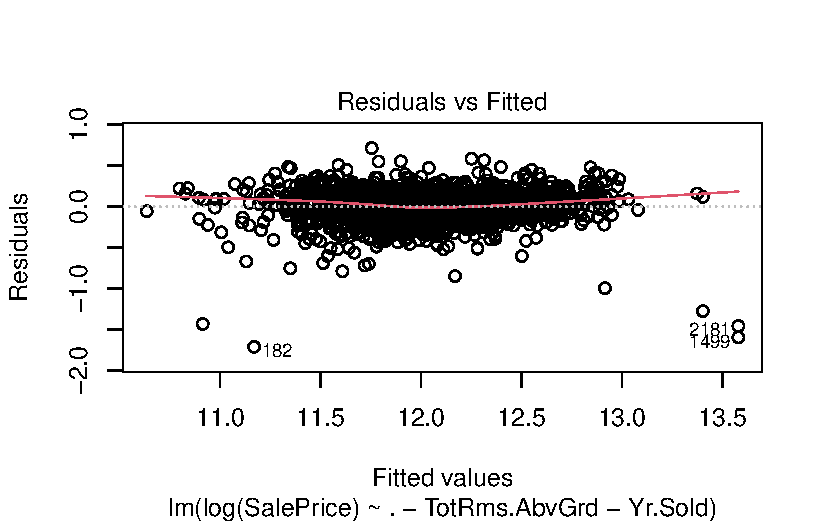
\includegraphics{paper_files/figure-pdf/plot1-1.pdf}

}

\caption{plot model}

\end{figure}%

\begin{figure}[H]

{\centering 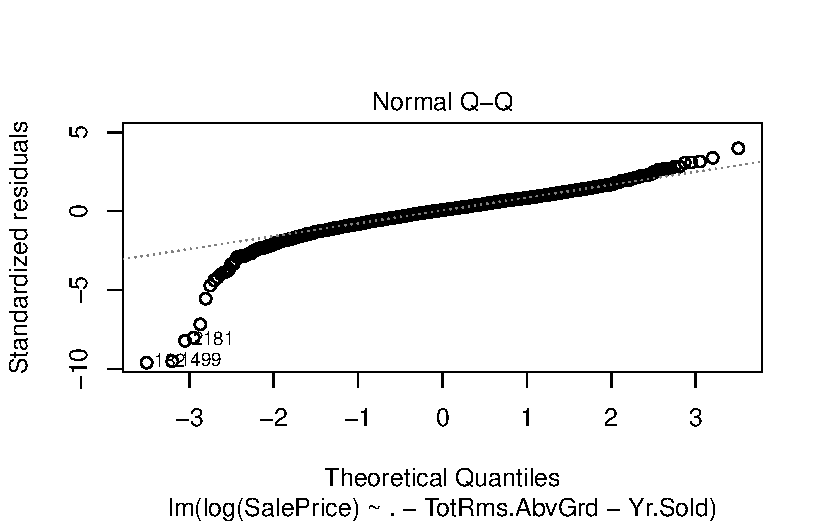
\includegraphics{paper_files/figure-pdf/plot1-2.pdf}

}

\caption{plot model}

\end{figure}%

\begin{figure}[H]

{\centering 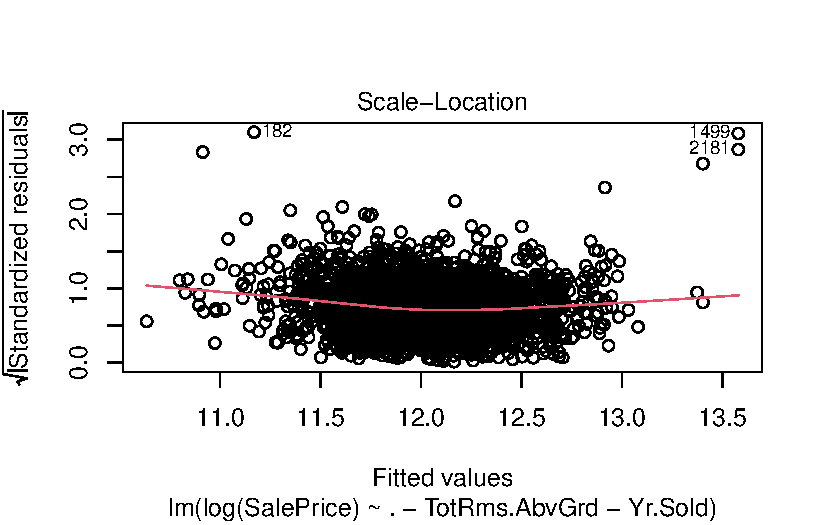
\includegraphics{paper_files/figure-pdf/plot1-3.pdf}

}

\caption{plot model}

\end{figure}%

\begin{figure}[H]

{\centering 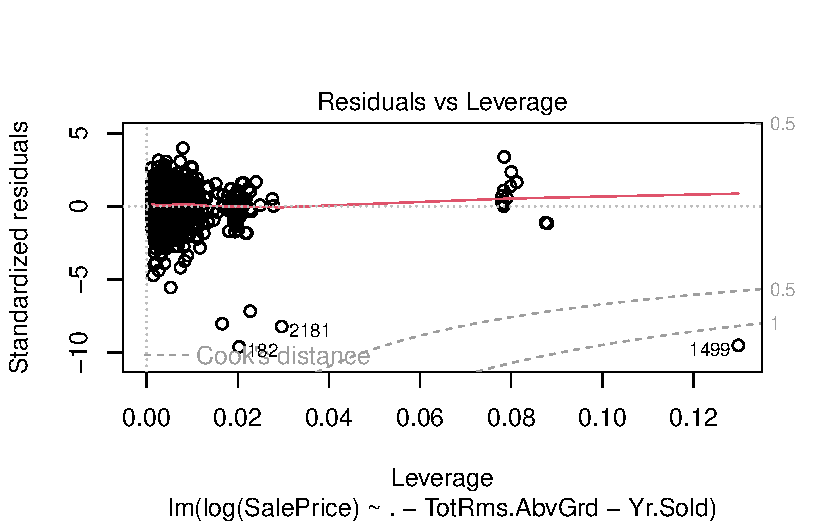
\includegraphics{paper_files/figure-pdf/plot1-4.pdf}

}

\caption{plot model}

\end{figure}%

\begin{verbatim}

Call:
lm(formula = log(SalePrice) ~ . - TotRms.AbvGrd - Yr.Sold, data = new_train)

Residuals:
     Min       1Q   Median       3Q      Max 
-1.04702 -0.08837  0.01205  0.10368  0.72952 

Coefficients:
               Estimate Std. Error t value Pr(>|t|)    
(Intercept)   1.052e+01  2.629e-02 399.959  < 2e-16 ***
Central.AirY  1.622e-01  2.087e-02   7.771 1.23e-14 ***
Lot.ShapeReg -4.749e-02  7.957e-03  -5.968 2.83e-09 ***
Garage.Cars   3.296e-02  1.230e-02   2.679  0.00744 ** 
Overall.Qual  1.319e-01  3.806e-03  34.657  < 2e-16 ***
Gr.Liv.Area   2.276e-04  1.064e-05  21.382  < 2e-16 ***
Garage.Area   3.237e-04  4.289e-05   7.547 6.73e-14 ***
Fireplaces    5.164e-02  6.616e-03   7.805 9.47e-15 ***
---
Signif. codes:  0 '***' 0.001 '**' 0.01 '*' 0.05 '.' 0.1 ' ' 1

Residual standard error: 0.1623 on 2009 degrees of freedom
Multiple R-squared:  0.8228,    Adjusted R-squared:  0.8222 
F-statistic:  1332 on 7 and 2009 DF,  p-value: < 2.2e-16
\end{verbatim}

\subsubsection{Model justification}\label{model-justification}

\begin{figure}[H]

{\centering 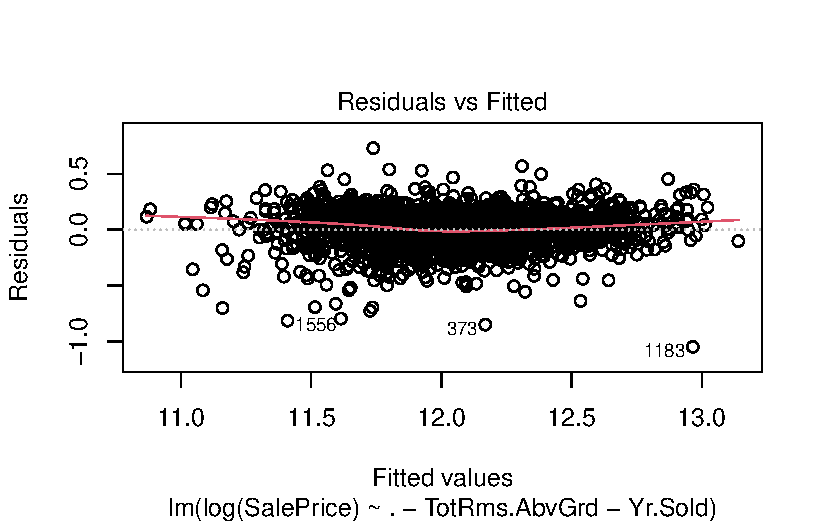
\includegraphics{paper_files/figure-pdf/plotmodel2-1.pdf}

}

\caption{plot model 2}

\end{figure}%

\begin{figure}[H]

{\centering 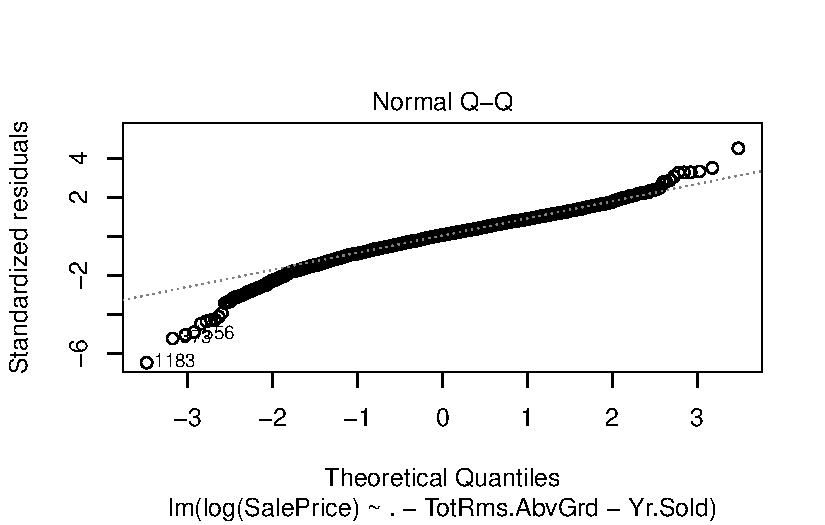
\includegraphics{paper_files/figure-pdf/plotmodel2-2.pdf}

}

\caption{plot model 2}

\end{figure}%

\begin{figure}[H]

{\centering 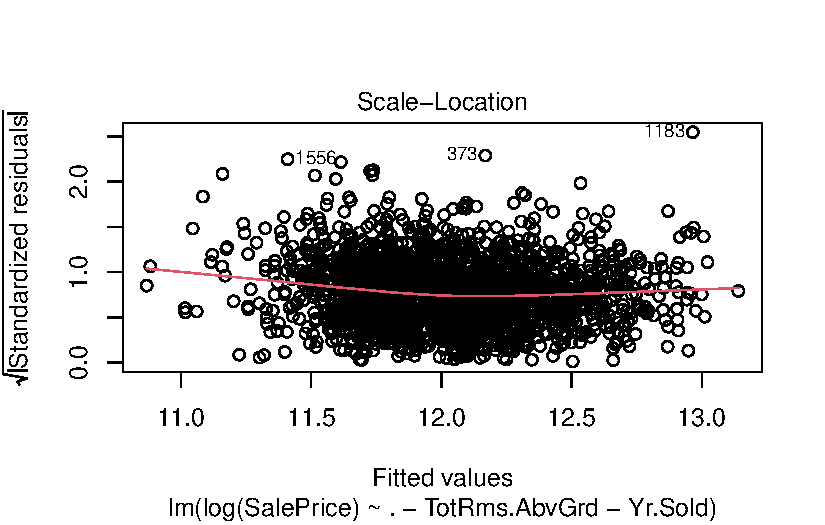
\includegraphics{paper_files/figure-pdf/plotmodel2-3.pdf}

}

\caption{plot model 2}

\end{figure}%

\begin{figure}[H]

{\centering 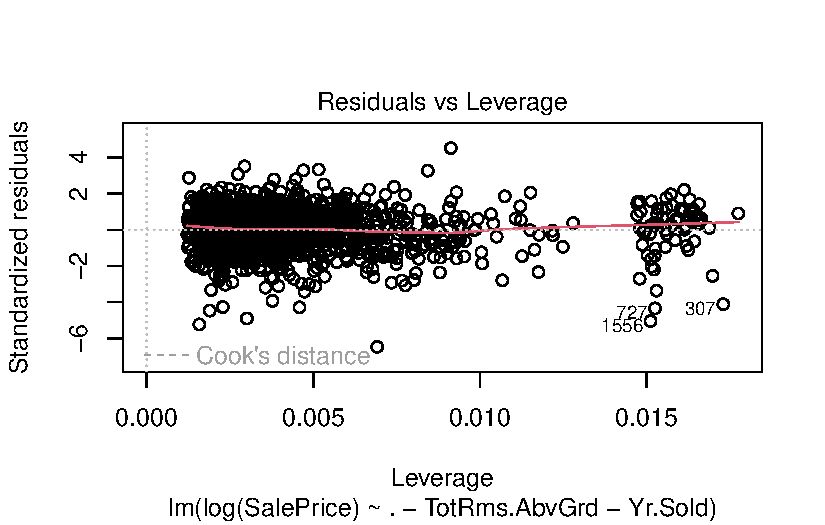
\includegraphics{paper_files/figure-pdf/plotmodel2-4.pdf}

}

\caption{plot model 2}

\end{figure}%

\begin{figure}[H]

{\centering 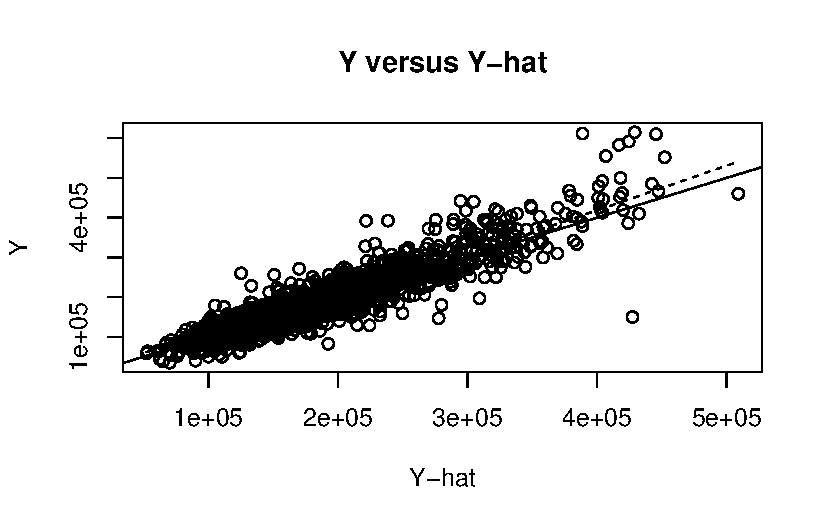
\includegraphics{paper_files/figure-pdf/plothat-1.pdf}

}

\caption{plot y hat}

\end{figure}%

\section{Results}\label{results}

\section{Discussion}\label{discussion}

\subsection{First discussion point}\label{sec-first-point}

If my paper were 10 pages, then should be be at least 2.5 pages. The
discussion is a chance to show off what you know and what you learnt
from all this.

\subsection{Second discussion point}\label{second-discussion-point}

\subsection{Third discussion point}\label{third-discussion-point}

\subsection{Weaknesses and next steps}\label{weaknesses-and-next-steps}

Weaknesses and next steps should also be included.

\newpage

\appendix

\section*{Appendix}\label{appendix}
\addcontentsline{toc}{section}{Appendix}

\section{Additional data details}\label{additional-data-details}

\section{Model details}\label{sec-model-details}

\subsection{Posterior predictive
check}\label{posterior-predictive-check}

\subsection{Diagnostics}\label{diagnostics}

\newpage

\section{References}\label{references}



\end{document}
